\chapter{Benchmark degli schemi omomorfici}

\section{Obiettivo del confronto}
Il capitolo precedente ha mostrato che uno schema omomorfico non viene scelto soltanto in base al livello di privacy desiderato. Tipo di dato, profondit\`a del calcolo, numero di slot e memoria disponibile influenzano la soluzione. I benchmark servono a rendere visibile tale costo.

La suite sperimentale confronta BFV, BGV e CKKS nella libreria OpenFHE. Il capitolo si concentra sui microbenchmark delle principali operazioni, in modo da mostrare come cambino tempo e memoria al variare dei parametri.

L'obiettivo non \`e stabilire una classifica assoluta. BFV e BGV lavorano su interi esatti modulo $p$, mentre CKKS lavora su numeri approssimati. Un tempo inferiore non rende uno schema adatto a un tipo di dato che non rappresenta correttamente.

\section{Ambiente sperimentale}
I benchmark sono scritti in C++17 e usano OpenFHE insieme a Google Benchmark. Il codice della suite sperimentale \`e disponibile in una repository dedicata \cite{benchrepo}. I risultati sono esportati in formato CSV e successivamente elaborati con Python. La macchina di prova ha le seguenti caratteristiche:
\begin{itemize}
  \item CPU AMD Ryzen 9800X3D, con otto core rilevati dal benchmark;
  \item 48 GB di memoria DDR5;
  \item ambiente Windows Subsystem for Linux;
  \item compilazione ottimizzata con \texttt{-march=native};
  \item uso di OpenMP nelle operazioni che supportano il parallelismo.
\end{itemize}

La creazione del contesto viene eseguita su un singolo core. Le altre operazioni possono sfruttare pi\`u thread. Il tempo riportato nei grafici \`e il tempo CPU medio prodotto da Google Benchmark. La memoria \`e una stima dell'heap osservato tramite l'allocatore di sistema; non include lo swap e deve essere interpretata come indicazione relativa.

\subsection{Parametri variati}
La suite varia due parametri:
\begin{itemize}
  \item la profondit\`a moltiplicativa, da circuiti molto brevi a configurazioni molto profonde;
  \item la ring dimension, da $256$ fino a $16384$ per il confronto comune, con valori superiori disponibili per BGV e CKKS.
\end{itemize}

BFV e BGV usano il plaintext modulus primo $p=786433$. CKKS usa una configurazione di scaling dedicata ai valori approssimati. Per le figure principali viene fissata una profondit\`a pari a 16, perch\'e consente di confrontare pi\`u schemi sulla stessa base e rappresenta un buon compromesso per molti scenari applicativi: non \`e troppo bassa, quindi permette calcoli non banali, ma non \`e nemmeno cos\`i alta da rendere il confronto poco leggibile e le operazioni troppo dispendiose.

\subsection{Avvertenza sulla sicurezza}
Nel codice dei tre benchmark il livello di sicurezza \`e impostato a \texttt{HEStd\_NotSet}. La ring dimension viene quindi forzata per studiarne l'effetto sulle prestazioni. Questa impostazione \`e utile per un esperimento controllato, ma non garantisce che ogni coppia di parametri raggiunga un livello di sicurezza standard.

I grafici non devono essere letti come raccomandazioni di configurazione. In un sistema reale il livello di sicurezza deve essere fissato e i parametri devono essere validati secondo le indicazioni della libreria e degli standard applicabili.

\section{Operazioni misurate}
La suite misura:
\begin{itemize}
  \item \texttt{ContextCreation}, cio\`e la costruzione dell'ambiente crittografico;
  \item \texttt{KeyGen}, per chiave pubblica e segreta;
  \item \texttt{EvalKeyGen}, per chiavi di moltiplicazione e rotazione;
  \item \texttt{Encrypt}, che cifra i dati con la chiave pubblica;
  \item \texttt{Decrypt}, che recupera il risultato con la chiave segreta;
  \item \texttt{EvalAdd}, che somma due ciphertext mantenendo il risultato cifrato;
  \item \texttt{EvalMult}, che moltiplica due ciphertext e consuma un livello;
  \item per CKKS, \texttt{BootstrapKeyGen}, che genera le chiavi necessarie al bootstrapping;
  \item per CKKS, \texttt{Bootstrap}, che rinnova un ciphertext per continuare il calcolo.
\end{itemize}

In forma intuitiva, se \texttt{Encrypt} produce due ciphertext che proteggono i valori $a$ e $b$, \texttt{EvalAdd} costruisce la cifratura di $a+b$, mentre \texttt{EvalMult} costruisce la cifratura di $a\cdot b$. Solo \texttt{Decrypt} rende leggibile il risultato finale.

Le misure sono microbenchmark: ogni test isola una singola operazione. Non includono trasferimento in rete, serializzazione, lettura dei dati o coordinamento tra attori. Sono utili per capire dove si concentra il costo, ma non equivalgono alla latenza completa di un'applicazione.

\section{Cifratura e decifratura}
Le Figure~\ref{fig:benchmark_encrypt} e~\ref{fig:benchmark_decrypt} mostrano rispettivamente il costo di \texttt{Encrypt} e \texttt{Decrypt} al crescere della ring dimension.

\begin{figure}[H]
\centering
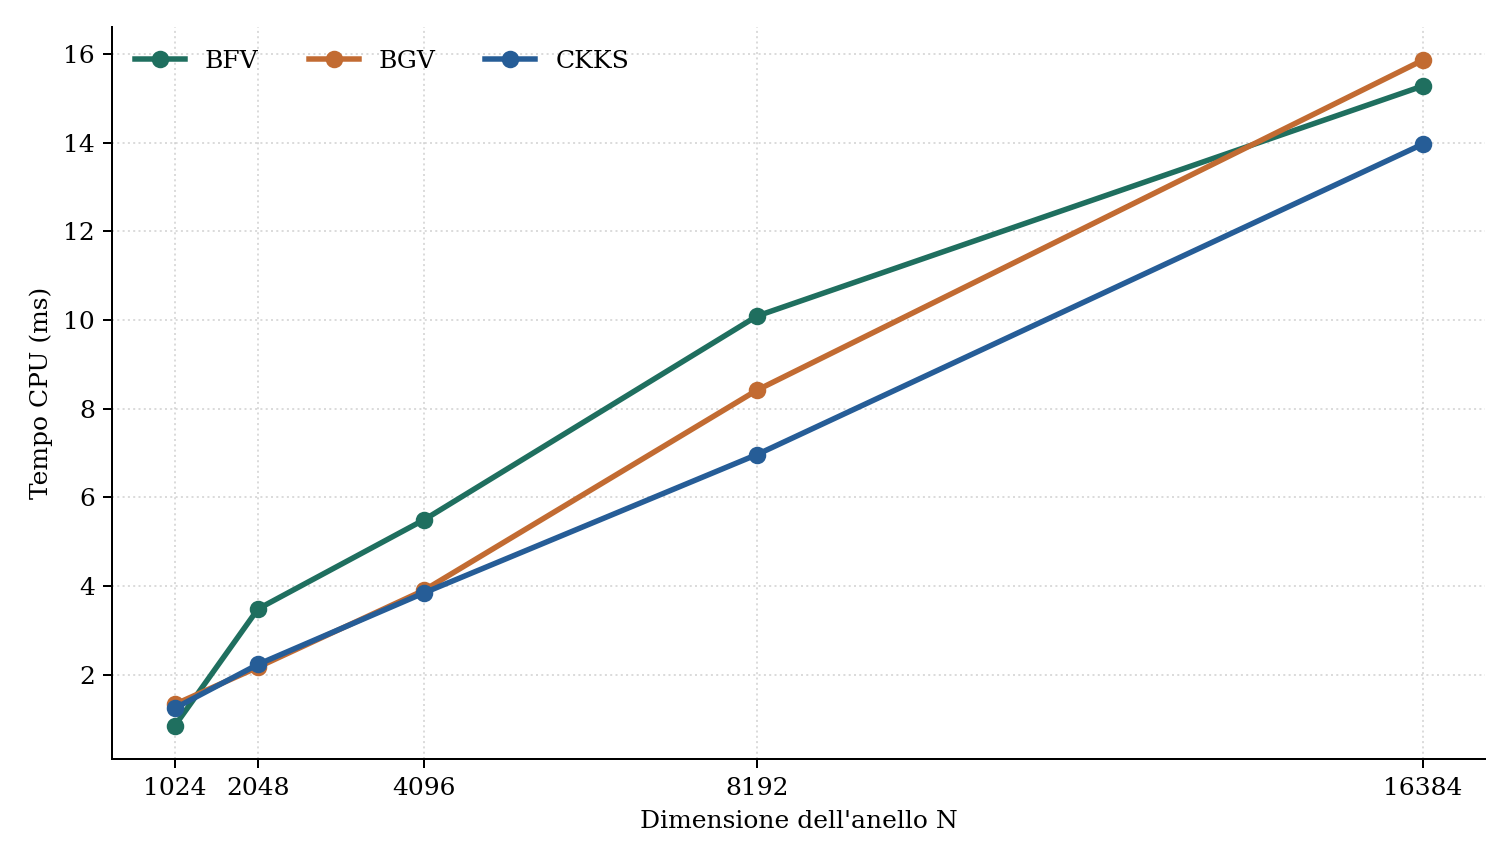
\includegraphics[width=0.64\textwidth]{figures/benchmark_encrypt.png}
\caption{Tempo di cifratura con profondit\`a 16.}
\label{fig:benchmark_encrypt}
\end{figure}

\begin{figure}[H]
\centering
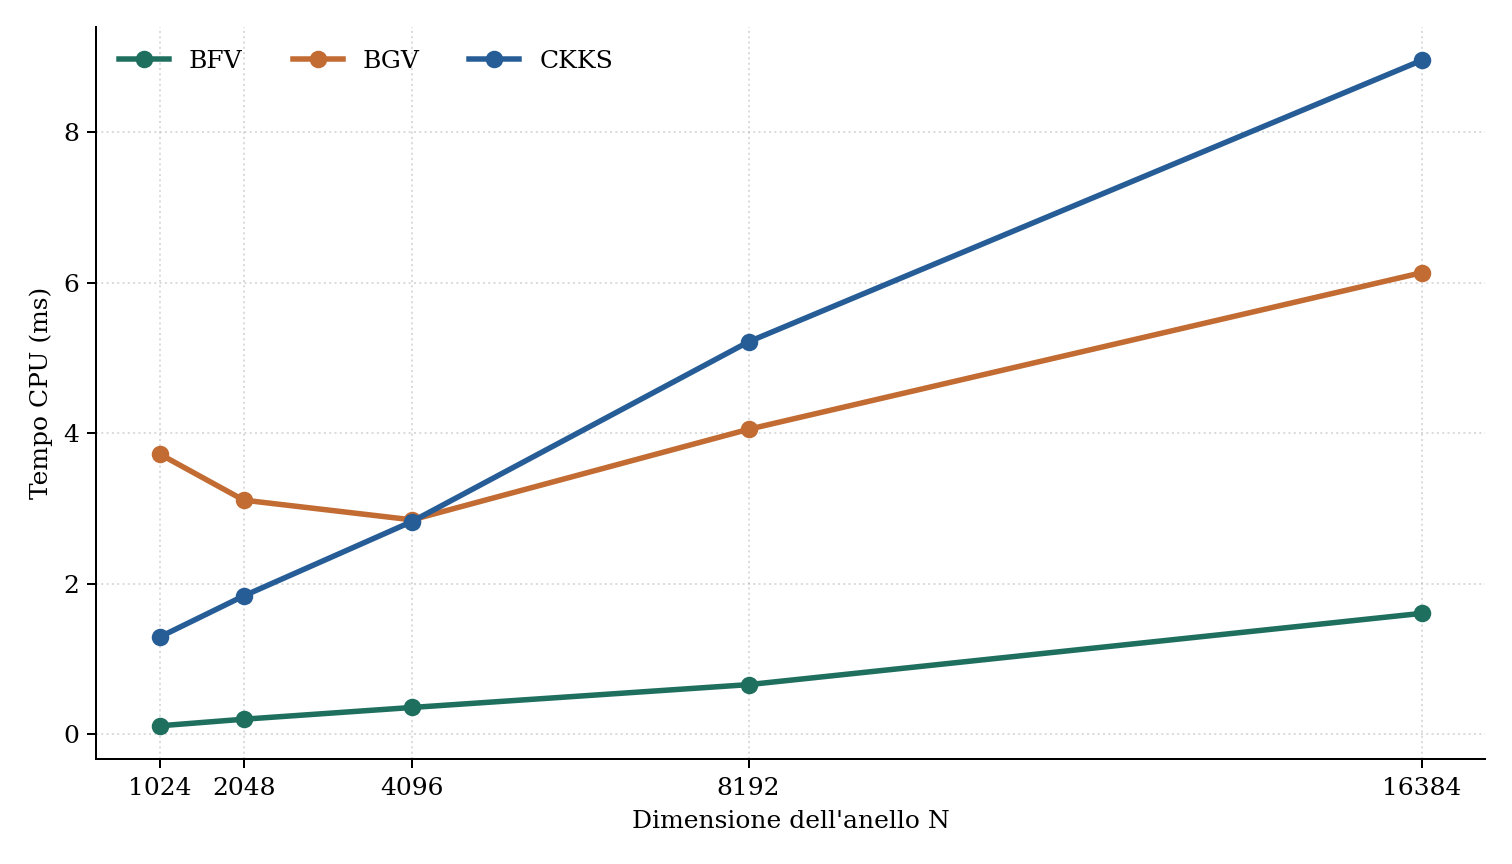
\includegraphics[width=0.64\textwidth]{figures/benchmark_decrypt.png}
\caption{Tempo di decifratura con profondit\`a 16.}
\label{fig:benchmark_decrypt}
\end{figure}

La cifratura cresce in modo abbastanza regolare con la ring dimension per tutti e tre gli schemi. Nel complesso, i tre andamenti restano piuttosto vicini: nessuno schema mostra un vantaggio netto e costante, e il grafico suggerisce soprattutto che il costo di \texttt{Encrypt} aumenta in modo simile al crescere di $N$.

La decifratura mostra invece differenze pi\`u nette. BFV resta chiaramente lo schema pi\`u rapido in tutto l'intervallo osservato. Tra gli altri due, CKKS tende a richiedere pi\`u tempo di BGV, soprattutto quando la ring dimension cresce. Il distacco principale, quindi, non \`e tra CKKS e BGV, ma tra questi due schemi e BFV.

Una dimensione maggiore offre anche pi\`u slot: BFV e BGV possono inserire $N$ interi, mentre CKKS inserisce $N/2$ valori complessi. Questo aumenta la quantit\`a di dati elaborabili in parallelo, ma rende anche pi\`u costose le singole operazioni.

\section{Somma e moltiplicazione}
Le Figure~\ref{fig:benchmark_add} e~\ref{fig:benchmark_mult} confrontano le due principali operazioni eseguite sui ciphertext.

\begin{figure}[H]
\centering
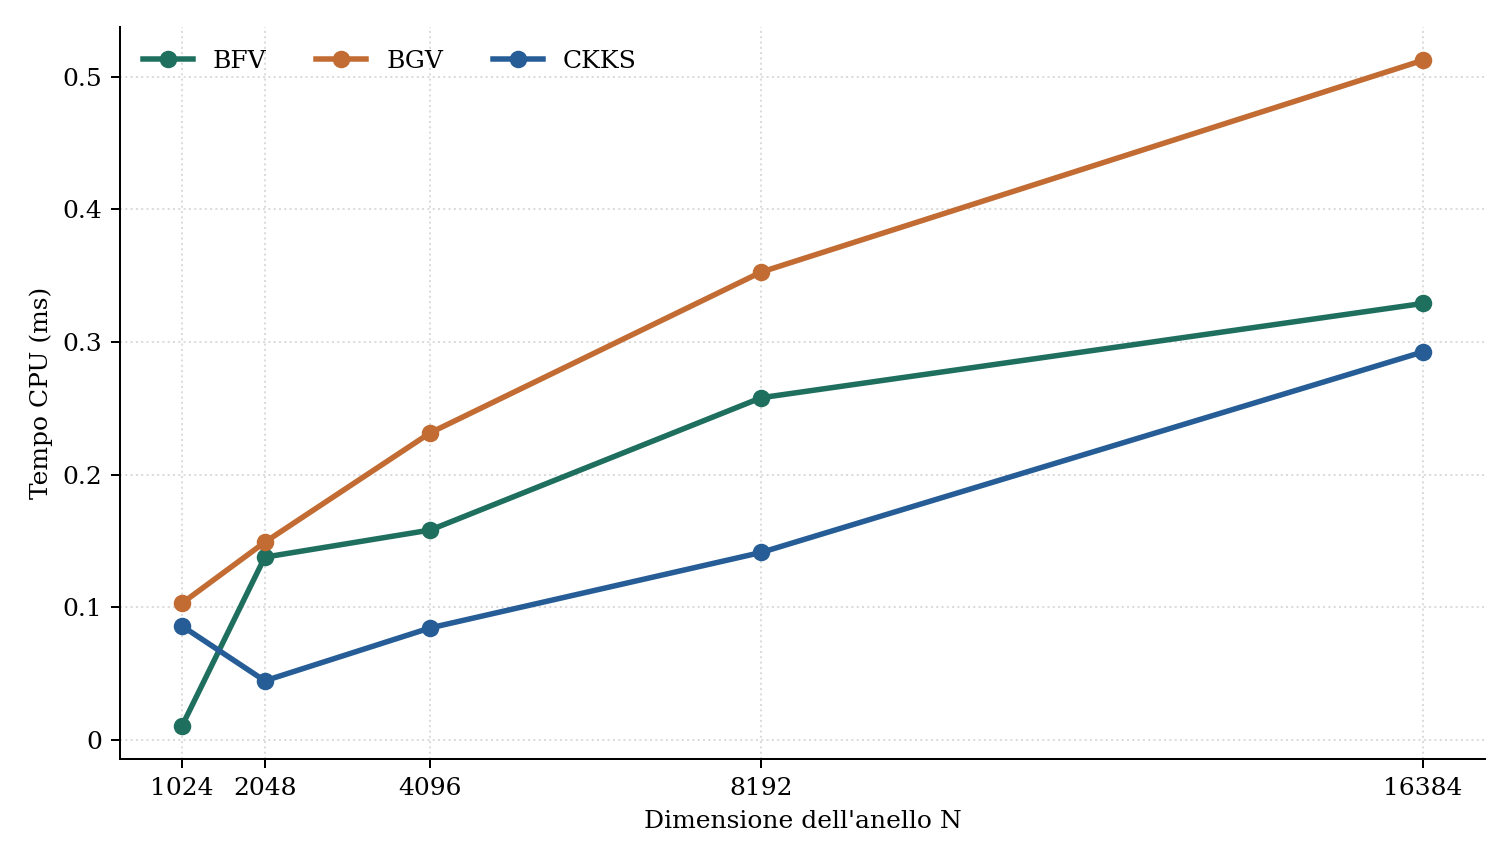
\includegraphics[width=0.64\textwidth]{figures/benchmark_add.png}
\caption{Tempo di una somma omomorfica con profondit\`a 16.}
\label{fig:benchmark_add}
\end{figure}

\begin{figure}[H]
\centering
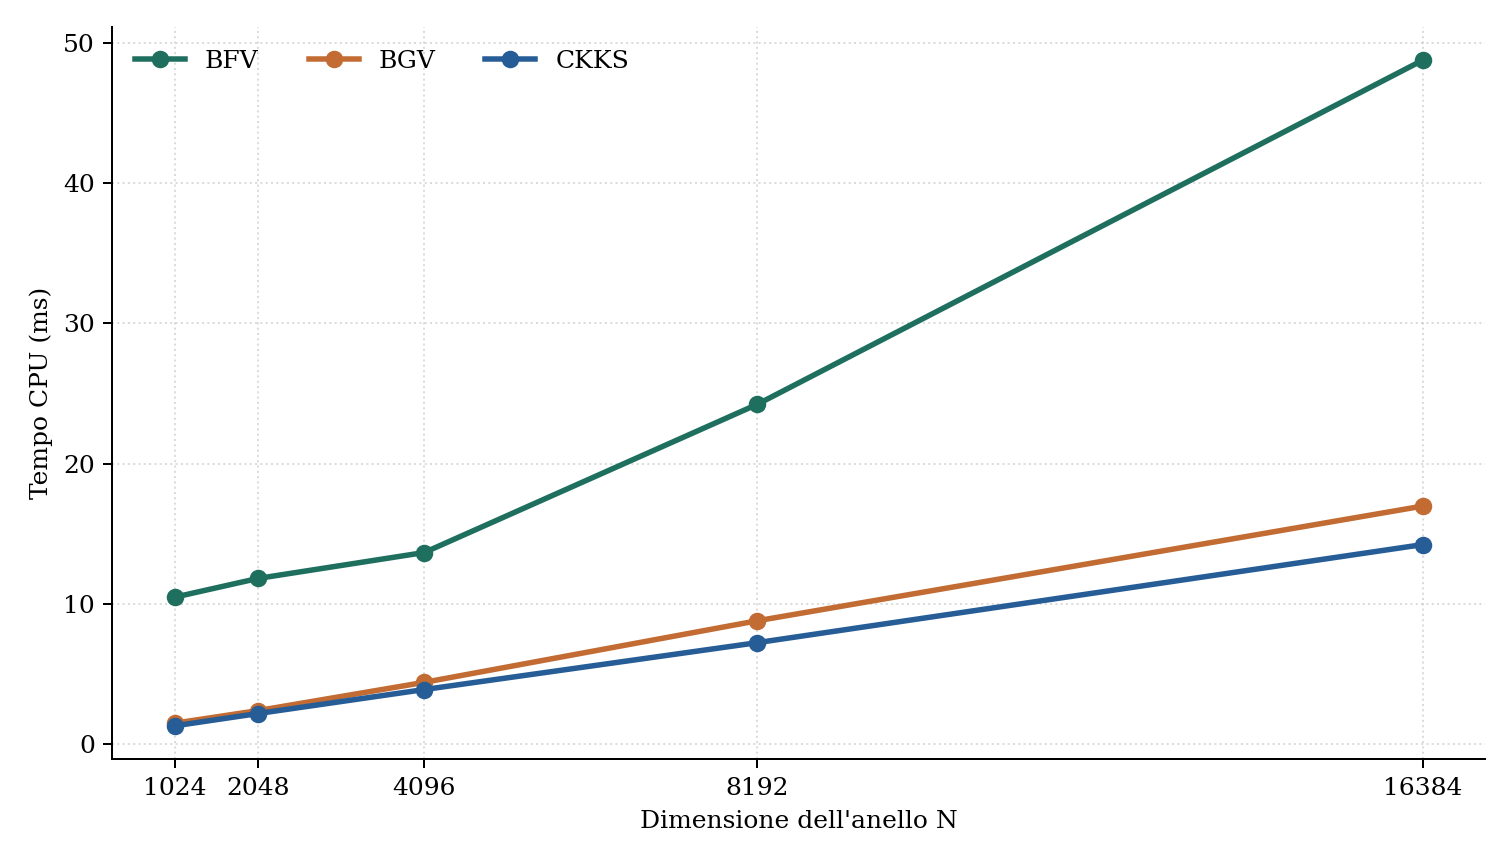
\includegraphics[width=0.64\textwidth]{figures/benchmark_mult.png}
\caption{Tempo di una moltiplicazione omomorfica con profondit\`a 16.}
\label{fig:benchmark_mult}
\end{figure}

La somma \`e chiaramente l'operazione pi\`u economica. I tre schemi restano tutti su valori molto bassi, con differenze contenute, anche se BGV tende a risultare un po' pi\`u pesante degli altri due. CKKS mostra l'andamento pi\`u leggero nel complesso, mentre BFV rimane vicino soprattutto nelle dimensioni intermedie e grandi.

La moltiplicazione cambia nettamente il quadro. Tutti gli schemi crescono con la ring dimension, ma BFV diventa molto pi\`u costoso di BGV e CKKS lungo quasi tutto l'intervallo osservato. Tra questi ultimi due, CKKS risulta in genere leggermente pi\`u rapido, mentre BGV gli resta vicino. Il dato principale che emerge dal grafico \`e quindi la distanza tra \texttt{EvalAdd} e \texttt{EvalMult}, e soprattutto il peso molto maggiore della moltiplicazione in BFV.

Le somme beneficiano del packing, che applica la stessa operazione a tutti gli slot. Quando invece il calcolo richiede controlli, prodotti tra valori o passaggi di machine learning, le moltiplicazioni diventano una parte importante della latenza.

\begin{table}[H]
\centering
\small
\begin{tabular}{lrrr}
\toprule
\textbf{Operazione, $N=4096$} & \textbf{BFV} & \textbf{BGV} & \textbf{CKKS} \\
\midrule
Cifratura & 5,496 ms & 3,906 ms & 3,846 ms \\
Somma & 0,158 ms & 0,232 ms & 0,085 ms \\
Moltiplicazione & 13,652 ms & 4,392 ms & 3,879 ms \\
Decifratura & 0,358 ms & 2,849 ms & 2,827 ms \\
\bottomrule
\end{tabular}
\caption{Tempi CPU con profondit\`a 16 e ring dimension 4096.}
\label{tab:benchmark_4096}
\end{table}

La Tabella~\ref{tab:benchmark_4096} mostra che una moltiplicazione costa molto pi\`u di una somma. Inoltre, le moltiplicazioni consumano livelli e richiedono evaluation keys. Il costo di una validazione omomorfica non dipende quindi solo dal numero di report, ma soprattutto dalla difficolta del circuito in cui essi saranno valutati.

\section{Memoria e interpretazione dei risultati}
La memoria registrata dalla suite non rappresenta il costo isolato del singolo ciphertext. Il processo mantiene contesto, chiavi e strutture create per il benchmark corrente. Inoltre, l'allocatore pu\`o conservare memoria tra operazioni. I valori devono quindi essere letti come impronta del processo e non come dimensione esatta di un oggetto.

La Figura~\ref{fig:benchmark_memory} mostra comunque la tendenza generale al crescere di $N$.

\begin{figure}[H]
\centering
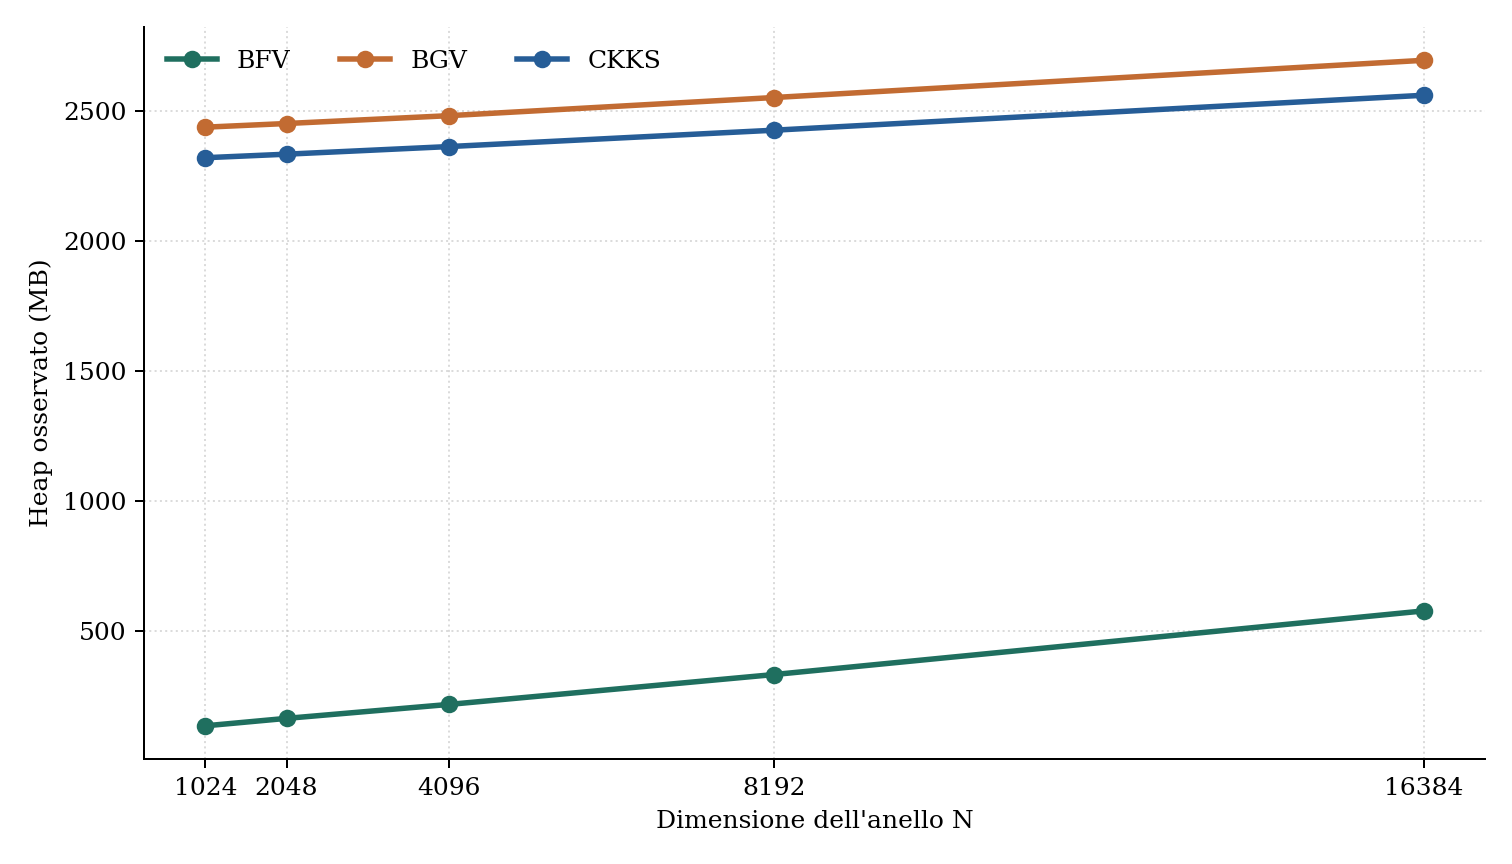
\includegraphics[width=0.64\textwidth]{figures/benchmark_memory.png}
\caption{Heap osservato durante la cifratura, con profondit\`a 16.}
\label{fig:benchmark_memory}
\end{figure}

BFV mostra nel processo di prova un livello di memoria molto inferiore rispetto a BGV e CKKS. I valori assoluti di BGV e CKKS includono memoria mantenuta dalla sequenza sperimentale e non devono essere interpretati come un confronto perfettamente isolato. La conclusione affidabile \`e pi\`u generale: contesti profondi, dimensioni maggiori ed evaluation keys possono richiedere gigabyte, rendendo la memoria un vincolo reale.

\section{Il costo particolare del bootstrapping}
CKKS include due benchmark aggiuntivi dedicati al bootstrapping. Il suo costo non dipende direttamente dal valore di profondit\`a usato, ma soprattutto dalla ring dimension. In pratica, aumentando $N$, anche il costo del bootstrapping cresce in modo evidente.

Questo rende il bootstrapping un'operazione molto pi\`u pesante delle somme e delle moltiplicazioni ordinarie. In calcoli poco profondi non \`e quindi conveniente, mentre diventa interessante soltanto quando serve proseguire un'elaborazione che altrimenti esaurirebbe i livelli disponibili.

Il confronto evidenzia una regola pratica: prima di ricorrere al bootstrapping conviene aumentare la profondit\`a, separare il calcolo in fasi o verificare se una configurazione leveled sia sufficiente.

\section{Scelta dello schema}
Se si vogliono usare numeri interi oppure aritmetica modulare, la scelta naturale \`e BFV o BGV. Tra questi due, BFV pu\`o andare bene quando il calcolo resta semplice, mentre BGV diventa in genere preferibile quando si usano operazioni pi\`u dispendiose della sola somma, in particolare le moltiplicazioni.

CKKS \`e invece la scelta adatta quando i dati non sono interi oppure quando si vogliono rappresentare numeri complessi. In questo caso bisogna accettare che il risultato sia approssimato e non esatto come negli schemi basati su interi.

\begin{table}[H]
\centering
\small
\begin{tabular}{p{2.3cm}p{3.2cm}p{3.2cm}p{3.2cm}}
\toprule
 & \textbf{BFV} & \textbf{BGV} & \textbf{CKKS} \\
\midrule
Dati & Interi & Interi & Reali o complessi \\
Risultato & Esatto modulo $p$ & Esatto modulo $p$ & Approssimato \\
Caso naturale & Conteggi e somme & Conteggi e controlli modulari & Statistica e machine learning \\
Attenzione & Overflow modulare & Overflow e profondit\`a & Precisione e rescaling \\
\bottomrule
\end{tabular}
\caption{Lettura applicativa dei tre schemi.}
\label{tab:scelta_schema}
\end{table}

\section{Limiti del benchmark}
I risultati sono stati raccolti su una sola macchina e in un ambiente WSL. Non sono presenti intervalli di confidenza tra esecuzioni indipendenti, misure energetiche o costi di rete. La memoria dipende dal comportamento dell'allocatore e dall'ordine dei test.

Il confronto usa parametri simili per rendere visibili le tendenze, ma gli schemi non offrono esattamente la stessa semantica. Infine, l'uso di \texttt{HEStd\_NotSet} impedisce di associare automaticamente ogni punto a uno specifico livello di sicurezza.

Questi limiti non annullano il valore dell'esperimento. I dati mostrano in modo chiaro che la ring dimension incide sul costo, che la somma \`e molto meno onerosa della moltiplicazione e che il bootstrapping \`e una fase eccezionalmente costosa. Sono proprio queste osservazioni a guidare le applicazioni dei capitoli successivi.

\section{Conclusioni}
I benchmark mostrano una tendenza chiara. Il packing permette di elaborare pi\`u valori in parallelo, ma dimensioni maggiori aumentano tempo e memoria.

Quando il sistema aggiunge moltiplicazioni, validazioni o training iterativo, il costo cambia sensibilmente. La profondit\`a e le evaluation keys diventano centrali; il bootstrapping deve essere usato solo quando necessario. I benchmark costituiscono quindi il collegamento tra le caratteristiche teoriche degli schemi e le scelte architetturali dei due casi di studio.
